%!TEX root = ../PhDThesis.tex



% *********************************************************************************************************************
\chapter{Discussion}\label{ch:synopsis discussion}
% *********************************************************************************************************************



\begin{revisedsubmission}[JR-5b, JR-3a,  ER-2b, ER-2c, ER-3a, ER-3b, ER-3c: New discussion focusing of the revised and clearer contributions of this thesis]
This discussion chapter will first turn to answering the research questions in this thesis by revealing: (1) an understanding of what constitutes a causal-social setting, (2) the nature of conversations that unfold within such a setting and the interactional projects that involve the use of devices, and (3) how this device use was interactionally organised in and through the ongoing conversation.

% he discussion  should  clearly  state  the  a)  substantive  contributions,  relating  to  the  body  of  work,  b)  the methodological contributions (e.g. differences in approach needed for different technologies / settings) and c)  the  conceptual  contributions  (e.g.  to  what  we  understand  about  collaboration,  what  settings  are considered in CSCW and how technology is characterised).This does not preclude the candidate developing the  design  implications  to  make  them  more  concrete,  but  if  they  are  to  be  included  they do  need  to  be substantially revised

Through this reflection, this discussion will synthesise and illuminate key aspects of the studies, including developing an understanding of the conduct in casual-social settings, reflecting upon the approach taken to the studies in this thesis, and raising insights for future design work.
Through reflection on these three points, this discussion will establish the thesis':
\begin{enumerate}
    \item \textit{Substantive} contribution through the presentation and discussion of members' conduct in casual-social settings and of how device use was involved in this interaction, relating to the existing literature introduced in this thesis (see \autoref{ch:background litreview}),
    \item \textit{Methodological} contribution in terms of practical approach (i.e. technology and setting) adopted in each of the three studies, and how the methodological validity is maintained, and
    \item \textit{Conceptual} contribution through the discussion on how collaboration unfolded, establishing the case for \ac{CSCW} to study casual-social settings, and for \ac{HCI} to examine design with \acp{VUI} for collaborative action further.
\end{enumerate}
\end{revisedsubmission}



% *********************************************************************************************************************



\crpagebreak\section{Conversation in casual-social settings}\label{sec:synopsis discussion conduct}
\begin{revisedsubmission}
This section brings together the empirical work in this thesis and reflects upon the findings in the scope of its overall research questions and objectives.
This thesis proposed the following research questions:
\PrintRQ{A}
\noindent and
\PrintRQ{B}

\noindent{}As described in the introduction, both of these questions serve as constituent parts of the overall objective that underpins the empirical work in this thesis, namely to identify:
\PrintRQ{overall}

\noindent{}This section discusses the various key tenets of this thesis: the notion of casual-social settings, the conversations that ensued within those settings, and the purposes for which device use was occasioned in and through the conversation and how this device use was sustained as part of this conversation.
This section forms a core component of this thesis' substantive contributions, by synthesising the notion of a casual-social setting and members' conduct within these settings, and how this relates to existing literature.
\end{revisedsubmission}


% *********************************************************************************************************************



\subsection{Casual-social settings}\label{sec:synopsis discussion conduct settings}
\begin{revisedsubmission}
This thesis took a pragmatic approach to understanding members' actions in casual-social settings by observing and examining groups of people socialising and interacting together.
The introduction of this thesis set out the notion of a casual-social setting (see \autoref{ch:intro}), and this was progressively developed throughout the empirical chapters (see \ref{sec:empirical pub design setting}, \ref{sec:empirical cafe design setting}, and \ref{sec:empirical home design setting}), with the work of members in those settings presented through the unpacking of empirical data.

The literature review in this thesis also discussed how the origins of designing for and studying collocated interaction in \ac{HCI} and \ac{CSCW} was within meeting rooms and control rooms.
As these fields \textit{turned to the social} (see \ref{sec:background litreview f2f turn-to-the-social}), designers and researchers embarked upon studying a range of ``centers of coordination''~\citep{Suchman1997} and later other settings such as public places~\citep{Weilenmann2002}, museums and cultural visiting locations~\citep{Ciolfi2003,Fosh2013}, and the home~\citep{Rooksby2015,Ferdous2016}.
This literature showed how the use of portable technologies has become ostensibly ubiquitous, with their use observed in all manner of settings as part of various activities.
Given the plethora of places in which device use has been identified as a recurrent activity, this thesis was not concerned with identifying further such places but in identifying the members' practices.% in relation to how such device use unfolds.
%Specifically, in the case of this thesis, the objective was to identify \textit{what} for and \textit{how} such use unfolded in situations where groups of people were conversing together in a casual and relaxed manner.

Therefore, the setting under study, not a specific location but rather a setting defined by the activity within, consists of a place in which people can gather to socialise, relax, and otherwise engage in an informal conversation. 
In this sense, the notion of a casual-social setting expanded upon work by others who have explored places such as social places and third places~\citep{Oldenburg1989}.
Such spaces were defined as pubs~\citep[pp. 88--108]{Fox2004} and caf\'{e}s~\citep{Laurier2008}, and non-home or non-work places~\citep{Oldenburg1989}.
In this thesis, the casual-social setting is, then, an amalgam of these definitions, with the underlying requisite for the selection of a place being that it be a place where members socialise together and relax as a group.

Interaction in three settings was empirically studied, in line with the three types of technology studied---that of touchscreen interaction with a portable device, \ac{VUI} interaction with a portable device, and \ac{VUI} interaction with a screenless smartspeaker.
The first study took place in a pub, a setting in which recent literature in \ac{HCI} had proclaimed an intrusion by the mobile phone~\citep{Su2015}, disrupting the activities within.
The second, a caf\'{e}, had also seen such claims, with authors such as \citet{Turkle2011} raising concerns about lost emotion and experience of places due to the use of devices.
In one case, for example, she highlights what she deemed a problematic situation in which she was with her daughter in a caf\'{e} in Paris, while her daughter used her phone to communicate with friends back home and thus was unable to experience Paris in the way she previously had~\citep[p. 156]{Turkle2011}.
The third setting, the home, had also seen criticism (for example, technology used during mealtimes being perceived as problematic by other family members~\citep{Rimer2009}).
Each of these settings was chosen as they were perspicuous~\citep[p. 181]{Garfinkel2002} to the study of conversation amongst groups of people where device use was known to unfold in such a gathering.
Indeed, as discussed, some literature has examined portable phone use in a variety of settings (see~\ref{sec:background litreview f2f}), yet few have attended to explicating the purposes for which device use is occasioned and how this use is practically accomplished during face-to-face encounters\footnote{The work of \citet{Brown2013,Brown2014,Pizza2016} being some of the few exceptions, as discussed in the literature review in \ref{sec:background litreview f2f}. None of these studies, however, approach the topic of specific social gatherings such as those examined in this thesis.}, beyond mere glossing of interaction as unfolding or extracting perceptions of it through \textit{a posteriori} methods; in other words, empirical data was nascent.

The first two empirical chapters, then, reveal how interactions in these three settings unfolded when the use of the device was done through touch-based interaction and through touch and voice-based interaction respectively. %, and highlighted how the groups being studied used the devices for various purposes in and through the conversation, and naturally accounted for such interactions with the device.
The third empirical chapter examined interaction that included the members' use of a third technology---a \ac{VUI} smartspeaker.
This technology was new at the time of the study and this thesis represents the first academic effort to study interactions with such a device from an ethnographic in-the-wild approach.
Smartspeakers are explicitly designed to be installed in a location, requiring mains electricity and a Wi-Fi connection for operation, and are pictured in marketing materials as being positioned in places such as a desk in an office, or in the home. 
Therefore, this study also took place in a perspicuous setting for this technology---a communal area in the home.

While this thesis is not the first piece of work to use the term `casual-social setting', with it applied to places for smokers~\citep{Schane2009}, hotel suites~\citep{Pigram1996}, college classrooms~\citep{Yamada1981}, and places where ``people can openly meet and interact with one another''~\citep[p. 42]{St.Lawrence1983}, it is seemingly the first attempt at explicating interaction in such a setting thus defined.
%To identify existing studies of interaction in such settings, one must turn studies of everyday interactions and gatherings, e.g. \citet{Goffman1968}'s work on behaviour in public places, or studies of iPhone use in everyday life~\citep{Brown2013}.
The empirical chapters in this thesis reveal how interaction in this sort of setting is replete with complex tasks undertaken to address members' needs, as part of the unfolding casual social interaction.
Indeed, this thesis delves deeper than existing literature by its focus on minutiae of interaction amongst groups to uncover members' interactional projects for which devices are used, and thus addresses the gap in relation to empirical data of device use.
%
% Certainly, recent literature in \ac{HCI} and \ac{CSCW} on interaction in such settings is nascent, and while the term casual-social setting is often used to refer to types of places, rarely is such a place defined.
% Furthermore, often studies of such settings are not closely studied to reveal what and how conversations unfold within, and how members of the setting draw upon technologies such as smartphones as part of their interactions.
The next section discusses the findings from the study of social interaction in such settings, using the data presented in this thesis.
\end{revisedsubmission}


% *********************************************************************************************************************



\subsection{Conversations in casual-social settings}\label{sec:synopsis discussion conduct conversations}
\begin{revisedsubmission}
This thesis was motivated by the plethora of literature in both the popular press and across multiple academic disciplines on social interaction and the influence of technology being present or used during face-to-face encounters.
The literature review (see~\autoref{ch:background litreview}) identified a lack of empirical data on \textit{what is actually done} when people gather to socialise, and this is the first consideration of this discussion, identifying the members' interactional projects in conversation that occasioned the device use.

For the first two studies, which took place in the semi-public settings of a pub and a caf\'{e}, participants were recruited as groups of friends to gather and socialise together.
In the third study, families were recruited as households to take part in the study, with the smartspeaker positioned in a communal place within the home.
With regard to the practices observed in the studies themselves, however, the device interactions that took place were occasioned by the members, without guidance or prescription of what should be done as part of the research.
In this sense, what was studied was unscripted and naturally occurring interaction within the setting.
In all three situations, the focus of the study was on the conversation that unfolded, and of the methodical ways in which device use was occasioned, interleaved, and oriented to within the interaction.
In other words, the focus was on the social interaction around the use of the devices, and not the use of the device itself.

Indeed, in each setting, conversations were shown to vacillate between topics, with new topics pivoted to in talk without resolution of prior discussions, e.g. in the resumption of conversation following device use in the pub (see \ref{sec:empirical pub findings contest}) or without clear antecedent in talk, as Susan proposes that the family play a game while eating a meal together (see \ref{sec:empirical home findings game}).
Conversations were also shown to go on in parallel to other discussions at the table, as separate conversational floors, e.g. as the friends have two separate but related conversations about animals with accents (see \ref{sec:empirical cafe findings answering}), or as two conversational topics interleave with each other, as members alternate between the topics, e.g. as the family make a joke about Liam eating his food amongst attempts to get the \ac{VUI} to start a game (see \ref{sec:empirical home findings game}).
Members were observed entering and leaving conversations, e.g. to get drinks (prior to the start of \ref{sec:empirical pub findings joke}), food, and to visit the toilet.

Additionally, in the observed studies members frequently made their device use naturally accountable by making the specifics of their device use observable and reportable\footnote{As introduced previously in \ref{line:naturalaccountability}, the \textit{natural accountability} of action is an accomplishment of members in the setting~\citep[pp. 1--34]{Garfinkel1967}}, e.g. by making a joke about something they read on their phone (see \ref{sec:empirical pub findings joke}), by rotating their phone around (see \ref{sec:empirical pub findings joke}), by making it visible to others (see \ref{sec:empirical cafe findings newinfo}), or by explaining their reasoning for using the device as they recall reading a news story recently (e.g. as Lily responds and confirms that she had read a story about animal accents (see \ref{sec:empirical cafe findings answering}).
This reinforces the perspicuity of device use in these settings: device use was not ostensibly treated as out of place in such a conversation, but rather as part of it, interleaved in---or occurrent alongside---conversation.
In other words, device use was treated by the members as part of, or rather \textit{embedded}, within the interaction in the casual-social setting.
Furthermore, through unpacking the methodical accomplishments of members, this embedded\textit{ness} is shown to be an interactional accomplishment \textit{as a result of} the practical work by members.

%I would argue that it was not merely encountered as embedded, members did practical work to embed the device, arguably, so this embeddedness is an interactional achievement. 

The use of devices was observed to be oriented as a matter to resolve the members' problems for which the device use was occasioned, e.g. through answering the question asked of the \ac{VUI} (see \ref{sec:empirical cafe findings answering}).
In this regard, device use was also shown to be accountably occasioned through talk so as to introduce new information to the conversation (see \ref{sec:empirical pub findings newinfo} and \ref{sec:empirical cafe findings newinfo}) and to contest an argument (see \ref{sec:empirical pub findings contest}).
Therefore, what this thesis has presented is empirical evidence to show that device use unfolds with members making their device use naturally accountable to co-present others.
The selection of these \textit{types} of settings was based upon literature (see \autoref{sec:background litreview society}) claiming that device use was occurrent during interactions in them.
The empirical data reveals how, as part of interaction in a casual-social setting, device use is certainly perspicuous, was made naturally accountable and, perhaps even, an \textit{acceptable}, practice by members.
Rather than glossing interaction as problematic, this thesis shows how members undertake interactional work to bring device use into interaction.
%This does not necessarily mean interaction with the device or the device user themselves is excluded from the conversation, however.
Device use was brought into the conversations in the setting, either as a topic or point of reference, or as a means of contributing to the conversation (e.g. as in the cases where the device use was used to find new information, see \ref{sec:empirical pub findings newinfo}) or to the device use.

In the second and third studies specifically, interaction with \acp{VUI} was occasioned by users as they establish and test the capability of the device as part of conversations about the device (see \ref{sec:empirical cafe findings capability} and \ref{sec:empirical home findings capability}).
\ac{VUI} smartspeakers, as per their design by manufactures, were also used for long running tasks, such as playing music in the background at a party (see \ref{sec:empirical home findings music}), or to play games together while having a meal at the dinner table (see \ref{sec:empirical home findings game}).
In the data presented in this thesis, members' projects involving the use of a \ac{VUI} device were shown to be interleaved with the ongoing talk amongst collocated others in the setting.
Furthermore, talk to the \ac{VUI} was made accountable to the members of the setting in and through the conversation, and indeed held to the same normative moral order as talk between interlocutors in the setting (see \ref{sec:empirical home findings music}).
In this regard, talk to \acp{VUI} is crucially shown to be part of the multi-activity home~\citep{Rooksby2015}, and unfolds alongside or interleaved within ongoing activities as an embedded activity in the home~\citep{Porcheron2018}.

Of course, not discussed in this thesis are moments where the device use unfolded for purposes of responding to notifications or checking the time, or solitary use of devices without others present.
However, this thesis did not set out to document all purposes of using technology in such a gathering, but rather, sought to explicate the interactional projects that occasion device use within a casual-social setting, and illuminate the naturally accountable ways in which this practice unfolded.

Summarily, interaction with all three forms of technologies turned upon both matters raised in the ongoing conversation in the setting and of those ostensibly unrelated to it.
Members occasioned device use as a topic in and of itself, or as a resource to address members' interactional problems in talk, such as information deficits or to answer questions.
The exhibits of data presented in this thesis demonstrably show how members treat device use within conversation as part of the activity of socialising as a group, rather than as a distinct activity.
The next section delves further into how this device use was occasioned and used in conversation in a casual-social setting.
%The next section explores how device use is accountably and interactionally organised within these settings.
\end{revisedsubmission}



% *********************************************************************************************************************



\subsection{Device use in conversation}\label{sec:synopsis discussion conduct device-use}
\begin{revisedsubmission}
The above section details the nature of what devices were occasioned for in conversation, in order to attend to members' interactional projects.
The final consideration here is of the how device use was brought into and used throughout conversation, and to make sense of how this was interactionally and accountably organised.
Each empirical chapter has presented the methodical accomplishments of how and why members used their devices (see \ref{sec:empirical pub summary methods}, \ref{sec:empirical cafe summary methods}, and \ref{sec:empirical home summary methods} respectively).
This section constructs an assemblage of these three chapters to reveal the practice of occasioning device use in conversation and how this device use is done during conversation.
This is not to demarcate or even regard these as distinct \textit{stages}, but to illuminate the ways in which device use is brought into conversation and accountably organised through it.
\end{revisedsubmission}



% *********************************************************************************************************************



\subsubsection{Occasioning device use in conversation}\label{sec:synopsis discussion conduct device-use occasioning}
In all three studies, members routinely occasioned device use in conversation by \textit{self-selecting to use their device}.
This was done to \iresubmission{contest arguments or answer questions posed in talk, or in the case of studying interaction around the use of touchscreen smartphones in a pub, also for remaining in touch with non-present others.
Moreover, in the studies in the pub and caf\'e, members had \iresubmission{conversations, such as about their favourite dog breeds (see \ref{sec:empirical pub findings newinfo})} or whether animals have accents (see \ref{sec:empirical cafe findings answering}), both of which led to a device being used to resolve the occasioned interactional project.
This echoes remarks by \citet{Brown2015} on the use of collaborative mobile search being a grossly observable feature of everyday interaction.
Even in the home, participants made use of \ac{VUI} smartspeakers for projects such as playing a game together while collocated around the dining table for a meal (see \ref{sec:empirical home findings game}), raising how technology ostensibly gets used during other ongoing activities in the home.}
%In these cases, the data presented in this thesis consists of exhibits in which device use is occasioned as part of conversation, by members of the setting using the device for a particular purpose within the ongoing interaction in the setting.}

Of course, members also \textit{selected others to use their device} as part of the interaction in a casual-social setting.
\iresubmission{With touchscreen device use, this was typically done as another member had a device accessible, and a member oriented to this by asking them to verify a fact using the mobile Internet (see \ref{sec:empirical pub findings newinfo}), an already identified use of portable devices in literature~\citep{Church2011}, although this thesis presents an empirical account of such an action.}
However, with voice-based interactions (i.e. both studies two and three), members \iresubmission{also turned} to asking others for assistance with \ac{VUI} input if they \iresubmission{ostensibly} suspected that the device would not be able to `understand' them.
%This selection relates to the definitions of `driving' interaction, unpacked in the explication of search on portable devices~\citep{Brown2015}.
%For example, in \autoref{frag:empirical cafe findings animals} from the study of \acp{VUI} on hybrid devices, Lily asks Karl to perform a request following the failure of the device to hear her voice:

In situations where the device use was occasioned in an ostensibly unrelated matter to the conversation, this was due to members \textit{attending to an interruption or notification from their device} (e.g. a message arriving or an alarm sounding that may have been configured during a prior interaction with the device).
%It was also common that their device use was \textit{seemingly incidental in nature}, and was accountably done as members checked for any missed notifications or the time, or even out of boredom~\citep{Church2012}.
It is this form of occasioning that has attracted some interest in literature \iresubmission{that addresses the impacts of technology use in society}, with many studies examining how systems might be designed to manage device interruptions and to select the most opportune moments to deliver notifications~\citep[see \ref{sec:background litreview society notifications}]{Fischer2011}.
This thesis offers little contribution to this space when these occasioned interactions were not brought into conversation \iresubmission{as this was out-of-scope of this thesis' objective in studying conversation in which device use was interleaved}.



% *********************************************************************************************************************



\subsubsection{Using a device in conversation}\label{sec:synopsis discussion conduct device-use using}
\iresubmission{People \textit{interleave their device use within the ongoing conversation}, and accountably accomplish this through various means, including shifting their gaze between their device's screen or putting their device down or picking it up (in the first two studies), or by \iresubmission{interleaving utterances directed at the \ac{VUI}} amongst talk to others in the setting (in the second and third studies).
The conversation that is interleaved amongst this device use included questions in relation to how to complete the task for which the device use was occasioned, e.g. clarification of the search terms to use (see \ref{sec:empirical pub findings newinfo}), to ask another person to help with the device interaction (see \ref{sec:empirical cafe findings answering}), or in relation to other matters of the setting, such as parenting (see \ref{sec:empirical home findings game}).}
As \citet{Brown2013} and others acknowledge, portable device use is part of the multi-activity of everyday life.
Just as in the study of device use and television watching, in which \citet{Rooksby2015} remarked that ``attention is accountably managed and organized in the course of watching [television] together''~\citep[p. 13]{Rooksby2015}, the findings in this thesis show that members' attention and orientation to device use is managed within a multi-party conversation in other casual-social settings too.
\iresubmission{In other words, the use of the devices was, in the same regard, identified as being accountably interleaved amongst the ongoing everyday activities by members as a part of those activities.}

\begin{revisedsubmission}
\paragraph{Accountable device use} \hfill \\
The notion of natural accountability is such that the members of this setting can both observe and provide a report on the action of others, and that those other members would recognise that report~\citep[pp. 1--34, see~\ref{line:naturalaccountability}]{Garfinkel1967}.
As discussed above, in the first study, members make their device use accountable through methods such as rotating their device, sharing the visibility of the devices' screen, or by verbally reporting the specifics for the use, reinforcing findings others have elucidated in relation to sharing activities using mobile phones~\citep{Raclaw2016}.
Although members can observe device use happening, and they can report for what ends the device use is happening as a result of its use in conversation, given the `private' nature of touchscreen-based device interactions (due to the small screen size), members cannot observe or report on the \textit{specifics} of what device use is unfolding (i.e. what the user is \textit{actually} doing).
In this, members rely upon the device user to make these specifics of device use accountable.

In the second study, members drew upon the same methods to account for the specifics of their device use, with members sharing the visibility of the screen by holding it between themselves and another person, or by verbally reporting on the outcome of requests.
As well as demonstrating the perspicuity of device use in these settings (discussed above in \ref{sec:synopsis discussion conduct conversations}), this also reveals the way in which members methodically and accountably organise this interaction.
\autoref{fig:synopsis discussion conduct device-use using accounting} below includes three examples from the first two studies of this practice of making the device use accountable through making the screen visible to another person:

\begin{figure}[bth]
    \subfloat[Leaning in to read the screen, from \autoref{sec:empirical pub findings newinfo}]
        {\label{fig:discussion embed accountable leaning}%
        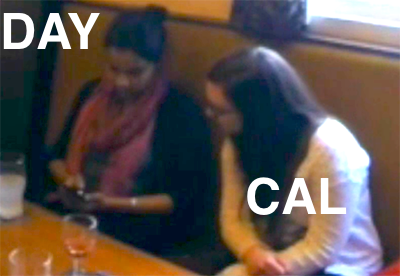
\includegraphics[width=.3\linewidth]{Graphics/3-1-Empirical-Pub/FragmentCollabSearch-2}} \quad
    \subfloat[Rotating the screen to show an email, from \ref{sec:empirical pub findings joke}]
        {\label{fig:discussion embed accountable rotating}%
        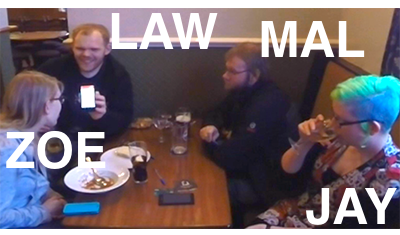
\includegraphics[width=.3\linewidth]{Graphics/3-1-Empirical-Pub/FragmentEmail-4}} \quad
    \subfloat[Sharing screen visibility to show failure of device to respond to voice, from \ref{sec:empirical cafe findings capability}]
        {\label{fig:discussion embed accountable leaning-2}%
        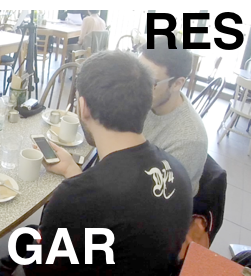
\includegraphics[width=.3\linewidth]{Graphics/3-2-Empirical-Cafe/FragmentMamma-2}}
    \caption{Examples from the first two studies of individuals making device use accountable by sharing visibility of the device screen.}\label{fig:synopsis discussion conduct device-use using accounting}
\end{figure}
\end{revisedsubmission}

\begin{revisedsubmission}
Furthermore, the specifics of input to the \ac{VUI} were hearable to those in earshot, as a result of interaction unfolding through talk to the device.
These requests to the \ac{VUI} device were occasioned in and through the conversation, and as a result of the hearable nature of the request and context within which it unfolds, members' requests are made naturally accountable (i.e. the specifics of the interaction with the \ac{VUI} are reportable as well as hearable).
For example, in the cases presented in \ref{ch:empirical cafe} there were conversations about animal accents, the time of sunset, and the capability of the \acp{VUI}, and each of these conversations established the context within which the \ac{VUI} request was made.
In other words, members' request to the \ac{VUI} was hearable as a result of it being delivered through talk, and reportable as a result of it being occasioned in and through conversation.
However, the responses from the \ac{VUI} typically defaulted to displaying information on the touchscreen of the device.
Members reported these responses either by providing a verbal or visual account of how the \ac{VUI} responded (e.g. showing the screen or verbally explaining the response), or through further \ac{VUI} interaction (i.e. if the device did not respond they would perform further address to the device, through which it is established the prior request `failed`).

%Although hearable to those in earshot, members accounted for their spoken input to the \acp{VUI} in and through the conversation, either before (e.g. as a `preparatory' account) or after the request to the \ac{VUI} was completed, or in response to being \textit{called to account} as a member responded to the device user's utterance to the \ac{VUI} (see \ref{sec:empirical cafe findings answering}).

In the third study, interaction with a \ac{VUI} smartspeaker was done entirely through voice and thus the specifics of their interaction with the device were hearable and made reportable, given that the use of the \ac{VUI} unfolded as part of the ongoing interactional project that occasioned its use (see~\ref{line:naturalaccountability}).
The talk to the \ac{VUI} was hearable through its utterance, and made reportable through its perspicuity to the ongoing activities in the setting (e.g. testing a new device in the home, playing music at a party, or playing a game together while eating dinner).
However, members did provide preparatory accounts in the home in instances where, for example, others were expected to play a game together using the \ac{VUI} (see \ref{sec:empirical home findings game}).
%Often, the hearability of talk to the \ac{VUI} and responses from the \ac{VUI} went some way to establishing the natural accountability of members' interactions with the device by making the specifics of those actions hearable.
In the three fragments of data presented, other members in the setting (i.e. those who were present for the \ac{VUI} use), were ostensibly able to recognise and practically reason about the interaction with the \ac{VUI} device through the requests to and responses from the \ac{VUI}.
This point is exemplified most clearly in instances where the user's request `failed', for example, and members collaborate on addressing the technical troubles with the \ac{VUI} without invitation or detail on the problem by the `original' \ac{VUI} user.
In this sense, the data demonstrates how members accountably recognise the initial request to the \ac{VUI} and the \ac{VUI}'s failure to adequately respond to that request, and practically reason and respond to it by taking further action, either by repeating or rephrasing the request (and, for example, often with different prosody).
In this, members did not explicitly report a failure of their request, as this was done through the use of the device, establishing its use as, perhaps, more `public' in nature.
\end{revisedsubmission}

A final note on this issue is to remark that, of course, members accounting for their device use is directly tied to the cohort and setting within which the device use occurs.
All the studies in this thesis focus on device use when people are with friends and family, and in a casual-social setting.
This links with the prior discussion above with regards to the rules of such a setting by establishing what is acceptable~\citep{Laurier2001}, and furthermore, it establishes the context in which the expectations for how to deal with situations where technology use occurs are managed:
\begin{quote}
    [T]here are many expectations about appropriate engagement with various technologies, including mobile phones---and more specifically texting on mobile phones---that are to do with how those particular cohorts organize their everyday affairs
    \quoteauthor{\citet[p. 262]{Tolmie2008}}
\end{quote}
In this, the practices explicated in this thesis represent and speak to the members of these settings, and this context is imperative to making sense of these findings.


\begin{revisedsubmission}
\paragraph{Collaborating on device use} \hfill \\
Members also included others in their interactional projects as a collaborative activity.
This either relied on \textit{assistance from others} such as guidance on what to search for, spelling (primarily study one), or verbal reports of the specificity of what was being done with the device.
It also relied on \textit{sharing control} of the task by multiple members being involved with the task either on the same device, or different devices~\citep{Brown2015}.

In the case of the first study, members always retained control of the use of their own smartphone by holding it in their hand, although, they did ask others for help with search terms (see \ref{sec:empirical pub findings newinfo}) or for performing requests to the \ac{VUI} if their device did not `understand' their pronunciation (see \ref{sec:empirical cafe findings answering}).
This suggests that the nature of \textit{personal} portable devices such as smartphones supports collaborative practices \textit{through invitation}.
In the second study, another co-present member attempted to complete the task on their own device as someone was struggling to use their \ac{VUI}, \textit{without invitation}.
Moreover, in the third study, featuring only shared \ac{VUI} devices, members self-selected to assist in completing members' interactional projects, again by `taking turns' to use the \ac{VUI} without invitation.

In this regard, interaction through voice, i.e. talk, remains the most obvious way in which members' conduct and use of devices is made recognisable and accountable to others, e.g. as part of the conversation.
With the accountability of device use, co-present members are able to \textit{recognise} and ostensibly self-select, without invitation, to involve themselves in the interactional project.
This led to members answering questions directed at \acp{VUI} (see \ref{sec:empirical cafe findings answering}), assisting with early termination of the \ac{VUI} response (see \ref{sec:empirical home findings music}), or assisting with the initial device user to complete their interactional project (see \ref{sec:empirical home findings game}).

\paragraph{Summary} \hfill \\
This ethnographic study has shown how members were able to interleave their use of devices in conversation to complete their interactional projects.
This rubs up against critiques others have made that suggest the use of---or even the mere presence of---devices in conversation have an isolating effect~\citep{Turkle2011}.
This thesis, through the adoption of an analytical lens that is 1) agnostic to the morals of actions and unaccountable factors, and 2) is used to reveal the accountable situated action of members within the setting, and shows how this interactional work was co-accomplished by members in the setting as \textit{part-and-parcel} of the face-to-face conversation.
In other words, \textit{members accountably attend to interleaving device use in conversation}, and that with the three technologies studied, this use was shown to be collaborative at times.
This collaboration turned upon the specificity of the device use being made observable and reportable\footnote{It was always recognisable to members of the setting that a person was \textit{using} a device, but only the use of a \ac{VUI} intrinsically makes the \textit{specifics} of that use hearable to those in earshot in---and naturally accountable through---its use in conversation.}, and with touchscreen-based interactions this was done through visual or verbal reports.
In the cases of talk to \acp{VUI}, the interaction itself was hearable and through its utterance as a situated action,  and made the specifics of the user's device interaction accountable to the setting as part of the interaction in the setting.
In turn, and any troubles with the technology that users experienced were attended to as matters concerning the occasioned interactional project.%, allowing members to respond to the specifics of the device use.

Through the presentation of empirical data, members' interactions with devices were interleaved amongst the conversation in each setting.
Members did this through occasioning the device in talk or through the conversation occasioning the device use.
They accounted for interactions with the device, engaged others in their device use through questions and requests for assistance, and ostensibly treated interactions with the device as part of the normative moral order within the setting.
The next section turns to discussing a crucial factor in relation to the observations that unfolded: the methodological considerations of this research.
\end{revisedsubmission}



% *********************************************************************************************************************



\section{Methodological considerations}\label{sec:synopsis discussion method}
\begin{revisedsubmission}
The objective of these observational studies was to understand how members practically attend to the matters of using a device in a multi-party conversation.
Accordingly, the analytic orientation of ethnomethodology was adopted.
Crucially, ethnomethodology provides the analytic lens to explicating the members' practical action and practical reasoning~\citep[p. 27]{Crabtree2012} to make sense of and reveal their methodical accomplishments as situated action (see \ref{sec:background approach em sequentiality}).

As the literature review established, this thesis is far from being the first piece of work to adopt an ethnomethodological orientation to studies of everyday life (see \ref{sec:background litreview f2f}), nor is it the first piece of ethnomethodological work to `create' the situation in which the study was to take place (i.e. participants were recruited to go to a setting, rather than the researcher going to a setting in which participants are already assembled).
For example, \citet{Suchman1985}'s work, Plans and Situated Actions, which has profoundly influenced \ac{HCI} and \ac{CSCW}-based studies of interaction, adopted an ``uncontrolled experimentation''~\citep[p. 114]{Suchman1985} approach to studying the use of an agent-based photocopier (see \ref{sec:background litreview f2f turn-to-the-social}).
In her work, although the basis for on participants were using the photocopier was a research study, participants' interactions were unscripted and unguided, or rather, ``uncontrolled''.
This is the overall approach taken with this thesis, insomuch that although participants were recruited to take part in a research study, there was no specific activity or task for participants to do, other than socialising together `as they normally would'.
The participants can assumedly be considered competent for this as they were recruited as families or groups of friends.

Although the analytic perspective adopted in this thesis was uniform across the three studies, the first two consisted of a video-recorded observation for ninety minutes, whereas the third consisted of contextual audio recording in the home over one month.
The study design decisions were based on the appropriateness, or perspicuity, of the device interaction that was of concern to the setting.
This section examines two key aspects that are relevant in terms of the methodological contributions of this thesis, namely the application of this approach in relation to the selection of settings perspicuous to the studies, and of the validity of the methodological choices taken.
\end{revisedsubmission}



% *********************************************************************************************************************



\subsection{Choosing a setting}\label{sec:synopsis discussion method setting}
\begin{revisedsubmission}
The first two studies in this thesis were video-based ethnographic studies.
Participants were recruited for the purpose of socialising as groups of friends who would usually socialise together in either a pub or a caf\'{e}.
This thesis follows in the tradition popularised in the \ac{CSCW} literature of studying the work of a specific setting, such as traffic control rooms~\citep{Bentley1992}.

In reviewing the progression of the development of \ac{HCI} studies, \citet{Grudin1990} remarks that:

\begin{quote}
    [There is] increasing preparation for the next outward step of the interface, into the social or work setting [\ldots] since most work occurs in a social context, computers will support it more successfully if they implicitly or explicitly incorporate social and organizational knowledge.
    \quoteauthor{\citet[p. 264]{Grudin1990}}
\end{quote}
In this, \citet{Grudin1990} provides the rationale for engaging in ethnographic studies of social settings in which technology use would eventually unfold, with ethnomethodology especially suited to this cause given its attention to the members' methodical accomplishments.
Furthermore, \citet{Heath1994} cautiously summarise what they called the ``lack of success of \ac{CSCW} systems'':
\begin{quote}
    [T]he lack of success of \ac{CSCW} systems derives not so much from their technological limitations, but more from their insensitivity to the organisation of work and communication in real work environments.
    \quoteauthor{\citet[p. 155]{Heath1994}}
\end{quote}
This thesis, of course, studies non-work settings, but given the now widespread use of devices in casual-social settings (see~\ref{sec:background litreview society}), there is an established case to undertake studies to reveal the details of the social organisation of interaction in everyday life settings, to support the design of technologies that are used within.
The rise of ubiquitous technologies ratifies the need to study everyday life in which these technologies are used—this is part of the \textit{turn to the social} (see~\ref{sec:background litreview f2f turn-to-the-social}).
\end{revisedsubmission}



% *********************************************************************************************************************



\crpagebreak\subsubsection{Choosing a public casual-social setting for portable device use}\label{sec:synopsis discussion method setting public}
\begin{revisedsubmission}
Ethnographic studies in \ac{CSCW} transgressed on to examining the particulars of everyday life, such as watching television~\citep{Rooksby2015} or families eating together at the dinner table~\citep{Ferdous2016}.
This is the work that this thesis methodologically follows.
A crucial factor that unfolds in all of the prior studies discussed, and that is fundamental to any ethnomethodological study (see~\ref{sec:background approach em comptency}), is the perspicuity of the interaction to that setting.
For example, concerning studies of how couples watch television together and use a mobile phone, it deductively follows to capture data in the main room of the home in which television watching occurs.
Likewise, it follows to examine the use of technology at mealtimes at family dinner tables.
To summarise, the site of the study naturally follows from the activity to be studied.

With this thesis, however, greater justification is given to the selection of settings because such a choice of setting is ostensibly less deductive. With the two video-supported observational studies, two public settings were chosen for the research to take place.
The type of setting was initially conceptually identified as a place where people gather and socialise together.
The settings of a pub and caf\'{e} were then selected for a variety of reasons (see \ref{sec:empirical pub design setting} for justification of a pub and \ref{sec:empirical cafe design setting} for justification of a caf\'{e}).
Summarily, however, there was already literature that revealed the social and relaxed nature of interaction in these settings, and of the device use in these settings.
Moreover, personal experiences of technology being used in these situations further influenced this decision.

The selection of these two settings required pre-negotiating access with business owners to ensure studies were able to take place and to ensure procedures were in place for dealing with inadvertent data collection of members of the public (e.g. people passing through the background).
However, while \citet{Rooksby2013} argues for such studies taking place in a lab-based setting, it was decided that  as there were not factors that needed to be controlled, and as there was no equipment or task other than socialising needed, there were no overriding benefits to running a pseudo-realistic lab-based study over running studies in an 'actual' setting.
Furthermore, obviously, others raise issues with this, remarking that laboratory studies are ``hardly the stuff of ethnomethodology''~\citep[p. 8]{Dourish1998a}, underscoring a need to get as close as possible to the phenomena of interest rather than reliance upon creating a simulated setting.
\end{revisedsubmission}



% *********************************************************************************************************************



\subsubsection{Choosing a home setting for VUI smartspeaker use}\label{sec:synopsis discussion method setting home}
\begin{revisedsubmission}
Given the underlying emphasis to study conversation around the naturalistic use of technology, and to ensure consistency with the first two studies, the third study took place in a setting perspicuous to the use of the device---the home.
Of course, \ac{VUI} smartspeakers were designed for places such as the home, and thus this outcome was straight-forward.
The challenges of studying interaction with new technology are, however, that users may not have competence in operating it.
In some experimental studies of new voice interfaces, for example, researchers have provided training (e.g. \citet{Molnar1996,Schaffer2015}) to ensure users' competency before an experiment with a \ac{VUI}.
The goal in this thesis, however, was to examine the interaction that unfolded around a device, not just with it, or as part of an initial encounter with the technology, or by following training or guidance on how to use the technology.
The goal was to understand how these technologies are used as part of routine interaction in the home. 
Therefore, to get closer to the phenomena of using these home-destined technologies, a more longitudinal approach to the study was necessitated.

As discussed previously within the empirical chapter concerning conversation around the use of \ac{VUI} smartspeakers (see~\ref{sec:empirical home design data}), this study relied upon audio collection only, and upon selective recording rather than continuous recording.
Given the longitudinal nature and the setting in which the study took place, these decisions necessitated careful consideration of how to capture data ethically, sensitively, and practically. Other approaches to studying technology in the home include repeated interview visits (e.g. \citet{Fuentes2019}) and diary studies (e.g. \citet{Forlizzi2007,Jokela2015b}), yet here there was an intent to actually understand the situated action of members that cannot be explicated through such methods.
Furthermore, although some studies of voice interfaces can rely upon self-reported logs of devices (e.g. \citet{Ammari2019}), given the need to examine interaction around the use of the devices this was not a practical method to adopt.
Others adopted methods such as relying on participants to start or stop recording devices before or after the interaction in a space or with a device, as previously done with portable device use during television watching~\citep{Rooksby2015}.
This would be problematic in this study as the use of \acp{VUI} can be started and finished in under a minute without much preparation.
Watching a television programme may consist of being within a specific space for thirty minutes or more, for example.
On the other hand, using a \ac{VUI} may take a matter of seconds with a user simply `passing through'.

Therefore, there was not a practical approach within the existing literature on how to accomplish the data collection for this study respecting the constraints outlined above.
To achieve the goal of this thesis, a specific recording device was designed and created for this purpose (and has since been released as open source software\footnote{See \url{https://github.com/MixedRealityLab/conditional-voice-recorder}}.) to selectively record interactions triggered by nearby users uttering a word.
This recording device (known as the \ac{CVR}) allows a longitudinal study to take place, in which participants learn (or not) how to use the \ac{VUI} within the home without guidance from researchers, in line with the prior two studies' approach of not guiding interaction with devices.
The \ac{CVR} is always `listening'---much like the \ac{VUI} smartspeakers---and retain the last minute of audio in memory.
When the programmed word is spoken, the device saves this prior minute and records for one further minute (extending this recording if the interaction with the device continues).

Furthermore, it allows for fewer data to be collected, to be done so ethically without capturing all matters of home life, and to not rely upon participants to manage their involvement in the study (i.e. members can focus their efforts on their normal mundane activities in the home as opposed to concerning themselves with the data collection).

The audio collected in this study provides a rich insight into the interactions in the home, in much (although not entirely) the same way as video data:
\begin{quote}
    [While video data] can form an archive, a corpus of data that can be subject to a range of analytic interests and theoretical commitments, providing flexible resources for future research and collaboration.
    \quoteauthor{\citet[p. 2]{Heath2010}}
\end{quote}
However, this brings with it a set of limitations, as \citet{Crabtree2012} elaborate:
\begin{quote}
    [Y]ou cannot see what people are doing alongside of the talk and there are circumstances where this may matter. [\ldots] Always be prepared to elaborate with notes the surrounding action that envelops the sequence of talk you are recording.
    \quoteauthor{\citet[p. 82]{Crabtree2012}}
\end{quote}
The approach in this study meant that fieldnotes also could not be taken as data collection was to take place over an extended period without a researcher present.
These two factors mean that this thesis presents only partial records of interaction in the home; however, given the parameters outlined above, and the focus being primarily interaction around the use of the \ac{VUI} device, this was seen as an adequate compromise.
What this situation means is that the data presented in this thesis comes with caveats, such as the inability to comment on conversations relating to the \ac{VUI} device away from the device, or matters that influence the \ac{VUI} use which unfold over a minute before or after interaction with the device.
These caveats limit the drawable conclusions this these can make with regards to commenting on the specific families' use of, and conversations about, different technologies in the home.
However, they do not preclude the examination of how their specific interactions with and around the device unfold \textit{in vivo} where it was recorded.
\end{revisedsubmission}



% *********************************************************************************************************************



\subsection{Methodological validity}\label{sec:synopsis discussion method validity}
\begin{revisedsubmission}
The approach that was taken in this thesis is not laboratory-based given the clear emphasis on selecting settings in which device use unfolded.
In the first two studies, the settings were pre-selected as part of the study design, the participants were all recruited as groups of friends to take part in the study.
In the third study, households were recruited as a family to take part in the study together.
The purpose of each study was described as one in which interactions with and around technology were to be observed.
Such an approach precludes conclusions of matters relating to why device interaction occurred as reasons of motivation, or other non-accountable factors.
These issues were disregarded in any case, given ethnomethodology's orientation to the naturally accountable activities of members only.
Therefore, this thesis' approach to studying the interactional minutiae of members' accomplishment reveals how and for what purpose \textit{in conversation} device use unfolded.

Moreover, in line with existing work in ethnomethodology on the notion of validity, this thesis does not pretend to demonstrate \textit{all the ways} in which \textit{all interactions with and around devices} might unfold.
This is a key tenet of ethnomethodological studies in that, through the presentation of the ethnographic record:
\begin{quote}
    [M]embers can recognise the work of a setting and also, as they are known and used in common, the machineries of interaction that they employ to accomplish and organise that work too.
    \quoteauthor{\citet[pp. 155--169]{Crabtree2012}}
\end{quote}
Thus, it is established that the work of producing the ethnographic report of members' actions is such that members can read and recognise the methods that are explicated.
This is because this record is constructed using the recognisable accountable practices of the members in the setting, rather than theorising about members' actions.
In this sense, this thesis presents the members' practical action and practical reasoning, rather than the analyst's theoretical reasoning.
The reliance upon only examining the accountable actions precludes the production of generalisable statements, but also underwrites the validity of the findings of this thesis.

In summary, this thesis selected settings which were perspicuous to the activity under investigation and recruited friends and families to take part in a research study.
Such an approach precluded discussing motivations for the device use that occurred, however, the analytic orientation of this thesis also precludes such a stance (given its emphasis on revealing the naturally accountable activities of members, rather than assembling a theoretical understanding of their actions).
It is from this regard of producing a record of accountable actions recognisable by members that establishes the validity of the approach taken in this thesis.
\end{revisedsubmission}



% *********************************************************************************************************************



\section{Insights for design work}\label{sec:synopsis discussion design}
\begin{revisedsubmission}[JR-5a, JR-5b, JR-3a, ER-2b, ER-2c, ER-3a, ER-3b, ER-3c, IR-4: Introduce the third discussion point. This is not to designate these points as implications for design but of matters that relate to design literature.]
This chapter's last reflection is upon how interaction unfolded across the three studies with an insight to supporting future design work.
Crucially, this chapter builds upon this thesis' methodological contributions to further examine members' conduct, to identify the collaborative efforts, and how \ac{HCI} and \ac{CSCW} might respond to these efforts.

This section will reflect upon the multi-party device interactions that unfold in each study, how this turns upon the accountability of device use, and how members collaborate as part of their interactional projects.
This will return to the case that the design and use of \acp{VUI} is made naturally accountable such that users can involve themselves in interactions collaboratively without invitation, and that this is of relevance to existing literature in \ac{HCI} to design collaborative systems for collocated interaction.
\end{revisedsubmission}



% *********************************************************************************************************************



\subsection{Collaborative device use}\label{sec:synopsis discussion design collab}
Previously, this thesis introduced work in \textit{mobile collocated interactions} \iresubmission{and \ac{HCI}}  which focused on the notion that device ownership will, in the future, occur with \textit{shared} devices, and that these devices will support \textit{multi-user} interactions that are \textit{collaborative}~\citep[see~\ref{sec:background litreview design mobilehci}]{Lucero2010d}.
Indeed, the findings of the empirical chapters in this thesis show that, in each of the studies and with each modality of interaction with a device, \iresubmission{members engaged in collaborative device use.}
\iresubmission{For example, with touchscreen interaction, members were observed collaborating, with one member  providing the query terms for a mobile search to be completed by another as part of the interactional project occasioned by their conversation (see~\ref{sec:empirical pub findings newinfo}).
In another case, one member proposed a rephrased request to the user of a \ac{VUI}, given that the members practically reason that the device `misinterpreted' the prior request (see~\ref{sec:empirical cafe findings newinfo}).
In a third case, the members of a setting took turns trying to start a game by issuing new requests to the \ac{VUI}, varying the prosody and words used in response to the failures of prior requests (see~\ref{sec:empirical home findings game}).}
This first case, for example, augments the existing literature that identified collaborative mobile search as an everyday task.
This examination by \citet{Brown2015} identified that there was
\begin{quote}
    [\ldots] considerable attention, effort and thought given to co-conversationalists while using a mobile device. Rather than shutting off conversationalists from each other, the devices become a site of investigation and discussion.
    \quoteauthor{\citet[p. 516]{Brown2015}}
\end{quote}
\iresubmission{This thesis extends this finding to encompass mobile device use for other purposes too, and how such practices unfold with both touchscreen device use and \ac{VUI} use, and that members bring this use into conversation in a casual-social setting.}
%This work provides numerous exhibits of multiple people collaborating to search for information using a mobile device in everyday life --- the interactionists studied may be occasioned by one member, but often multiple people are brought into the interaction through the embedding practices discussed above (see~\ref{sec:empirical pub discussion coop}).

Portable devices such as smartphones are inherently personal in their design and use~\citep{Lucero2010}, engendering `private' use \iresubmission{whereby even if co-present others are aware of---and can observe---device use unfolding, they often cannot observe or report on the \textit{specifics} of that use (e.g. they might not have a line of sight).
This is due, in part, to the relatively small size of device screens which inhibit greater visibility of the screen by those who are present beside the user.
Attempts to disrupt this private nature of device use have included adding large screens to settings to encourage users to share content from devices~\citep{Lucero2012}.}
However, the findings from the first study show how \iresubmission{devices are used as part of collaborative efforts by members, by the user asking others for assistance in completing their interactional projects, irrespective of the small size of the screen, or by making the screen visible to others.}
As they did this, they \iresubmission{made the device interaction accountable to others the setting, revealing the specifics of what was being done with the device, and thus transformed the `private' device use to one where the specifics of that device use were observable to \textit{some} others (i.e. this was not `public' use, however, as the screen may have been made visible only one other member).}

\begin{revisedsubmission}
%As discussed above, through conversation, members accounted for their interaction with their touchscreen devices (see \ref{sec:synopsis discussion conduct device-use using}).
Following the reflection of the findings from the first study, this thesis posed the question of how the practices of device use could unfold when the interaction mode was augmented with voice input (see~\ref{sec:empirical pub summary}), given that in such cases the talk to the \ac{VUI} would be hearable to those in earshot, making the specifics of users' actions hearable.
In particular, this outlook asked how members would use a \ac{VUI} as part of a gathering in a casual-social setting (see~\ref{sec:empirical pub summary outlook}).
As \citet{Crabtree2012} remark:
\begin{quote}
    [T]alk is the most obvious and pervasive way in which members conduct their work and make whatever it is that they are doing into an intersubjectively recognisable and naturally accountable activity.
    \quoteauthor{\citet[p. 44]{Crabtree2012}}%[p. 44]
\end{quote}
\end{revisedsubmission}
The second study addressed this matter and revealed how members' talk to devices, as interleaved within conversation, \iresubmission{made the specifics of their actions reportable, with the performance of the request organised within the organisation of the conversation in which the device use was occasioned}.
Additionally, this study brought to the fore that by switching the interaction mode of the device to voice as well as the use of the touchscreen, members ostensibly \textit{self-selected} to involve themselves with ongoing device tasks.
For example, they chose to perform requests on their own device if another member was struggling (see \ref{sec:empirical cafe findings newinfo}), or they offered assistance to the member to help diagnose problems (see \ref{sec:empirical cafe findings answering}).
\iresubmission{In this sense, device users did not necessarily account for the specifics of their device use, because their specific input to the device was hearable and made accountable through coherence with the ongoing conversation in the setting.
The action of uttering a request to the \ac{VUI}, in turn, was shown to occasion other members' self-selecting to respond to the device user's request (in other words, talk to the device was responded to by other people who were not the recipient of the utterance).
However, members provided accounts, especially to provide the details of the response from the \ac{VUI}.
At times these accounts were implicit made by members (i.e. when a member uttered a subsequent identical request, through which they establish the failure of the previous request).
At other moments, it included members explicitly confirming the success or failure of the \ac{VUI} to respond to the request.
In this, through the utterance of the request, the device interaction with the technology becomes `semi-public', insomuch that members' requests to the \ac{VUI} were made naturally accountable through their use as part of the social interaction in the setting, yet members were relied upon by others for verbal or visual reports of the \ac{VUI}'s responses given that these responses were displayed on the device touchscreen.}

%These findings showed how completion of the task was, in a sense, \textit{democratised}, by the switch to voice interaction, as the control of the completion of the task was removed from the device user and became managed through the conversation and social order of the setting (see~\ref{sec:empirical cafe discussion multiparty}).
%However, although the completion of the task was democratised, members still retained some control over interactions---they were relied upon the user(s) to report messages displayed on the screen, or to read information that had been found, for example.


The third study moved this examination into the realm of interaction through voice only, and where the technology under study became a shared device in the home.
As such, although the observations in the study of \acp{VUI} on portable devices explicated the hearable nature of the request made to the \ac{VUI}, and its coherence to the conversation establishing its natural accountability, in the study of voice-only interactions, the findings reveal how all members of the setting could orient to and attend to matters of the device interaction.
The hearable nature of requests was again revealed, with members' requests being explicitly held to the normative moral order by those in the setting (see \ref{sec:empirical home findings music}).

\iresubmission{Furthermore, with these interactions, the response was hearable, \textit{and reportable} through the coherence of the accountable request and ongoing conversation in the setting that occasioned the original request.
This natural accountability of the response, and the shared and public nature of \ac{VUI} smartspeaker in contrast to a portable smartphone, has the further consequence that all co-present members can not only respond to the request, but can also respond to the response from the \ac{VUI}.
This was seen as members respond to the \ac{VUI}'s response and make successive requests in accord with the prior one, e.g. in ratcheting up the testing of the \ac{VUI} (see~\ref{sec:empirical home findings capability}), or as members take turns attempting to start a Skill  (see~\ref{sec:empirical home findings game}).
In these cases, no member could retain control over the device and the `politics of control'~\citep{Porcheron2018} were managed through the social order of the home\iresubmission{, as part of interaction in the home between those who are present.
In some cases, members were called to account for interaction with the device that another member deemed out of place for the setting (see~\ref{sec:empirical home findings music}), but in this situation, it was not the purpose of the device interaction at hand, but the use of language involved that was remarked upon as being deemed problematic.
What the data in this thesis shows is that the use of a \ac{VUI} smartspeaker, as occasioned by conversation, unfolds as a `public' activity, whereby the specifics of that use are hearable and reportable to those who are co-present.
The data shows crucially how this use is regulated through the social order of the home as an accomplishment of the members in the home.}

\begin{revisedsubmission}
Through the careful reflection on members' conduct and how they accomplished their collaborative efforts to complete the occasioned interactional projects, this section has identified collaborative action amongst members in such settings, and this establishes the case for further studies in \ac{CSCW} to critically examine the nature of studying interaction in such settings.
Some literature has examined this (as discussed above, see~\ref{sec:synopsis discussion conduct}), but crucially, what this thesis shows is how there is further cause to examine such settings to reveal the collaborative efforts within, to support design work.
Although the definition of a casual-social setting was broad, as a concept it builds upon the work of others who have called for ethnographic studies of social settings~\citep{Grudin1990}.
The need to study the organisation of interaction of settings in which technology is to be used collaboratively is well rehearsed (e.g. \citet{Crabtree2009,Heath1994}), yet the work in this thesis suggests that such technology was shown to be deficient in meeting members' needs, e.g. multiple interactional projects were left unresolved. %\footnote{Of course, this thesis argues that the non-resolution of prior conversational topics is part of interacting in a casual-social setting, yet this thesis still proposes that technology \textit{could} meet these needs such that members need not abandon an interactional project.}.
Nevertheless, as this thesis has argued, members undertake interactional work to account for and accomplish this collaborative effort and the `need' to `successfully' complete an interactional project ostensibly does not exist in a casual-social interaction, therefore \ac{CSCW} should take the opportunity to identify ways to ameliorate these challenges through further ethnographic work.
The concept of a \textit{casual-social setting} is established around the notion of members' conduct, and this thesis has unpacked three such studies of that.
Members' conduct is, of course, cohort dependant (see~\ref{sec:synopsis discussion conduct device-use using}) and thus, further studies are needed to reveal more about the interactional projects, and ways in which members' problems are addressed with technology.
The next section further reflects upon these responses from the \ac{VUI} and how the collaboration that unfolded turns upon them.
\end{revisedsubmission}



% *********************************************************************************************************************



\subsection{VUI responses as supporting further action}\label{sec:synopsis discussion design vuiresponses}
\begin{revisedsubmission}
This final discussion section examines an area of concern for \ac{HCI} in the challenge of designing interfaces to support collaborative action amongst members of the setting.
Collaboration, as discussed above, unfolded as an interactional accomplishment in each setting, as members worked together to complete their occasioned projects.
With the latter two studies, however, this collaboration ostensibly turned upon the hearable nature of the interaction with the device.
This section critically examines how this interaction could be further examined, linking to existing publications in \ac{HCI}, to design interactions that meet members' interactional needs.

In reflecting upon the study of \ac{VUI} smartspeakers in the home, \ac{VUI} interaction is shown to consist of the form \textit{request to \ac{VUI}-response from \ac{VUI}}.
At times, and in all the cases of \ac{VUI} device in the home presented in this thesis, a response from the \ac{VUI} is followed by successive requests by the members of the setting.
Through the analysis, the \ac{VUI} responses themselves are analysed by members for the `account' of sorts they provide on the state of the \ac{VUI} device, and its processing of the previously made request, i.e. the response (or not) of a failed request occasioned members to practically reason and perform further actions to accomplish the interactional project.
The data from both studies two and three suggest a level of inadequacy of some responses \textit{as resources} to furnish this analysis to proceed with the interaction.
Consider how members in the third study fail to start the Beat the Intro Skill due to the repeated non-obvious source of technical trouble (see~\ref{sec:empirical home findings game}) before the device ultimately provides a response to a request that includes a partial transcription of the user's spoken words, and the \ac{VUI} offers a next candidate action.
This action provides a mechanism to practically reason about the processing of the voice-only device.
Of course, with touchscreen-based devices, this mechanism for users to reason about \ac{VUI} troubles was provided through messages displayed on the touchscreen, but these were only known to others if the device user `made them available' by reporting them (verbally or visually).

This thesis argues that the accountable nature of a `verbal' response from a \ac{VUI} smartspeaker is used as a resource by the original \ac{VUI} user, and other co-present members, to make successive requests.
It is through the natural accountability of members' successive requests to the \ac{VUI}, and how these turn upon the response from the \ac{VUI}, that reveals the practical reasoning of multiple members, collaborating to complete the interactional project.
Members demonstrably show reasoning about failure through a discussion in conversation (see~\ref{sec:empirical cafe findings newinfo}), or through repeated utterances to the device by different members with different prosody (see~\ref{sec:empirical home findings game}).
In both cases, it was this natural accountability of the response, established through the ongoing work of the setting, that provided the resource for further action.
\citet[p. 10]{Porcheron2018} term this characterisation of responses as ``resources for further interaction''.
In examining interaction in a multi-party setting, this resource is established as supporting further interaction by  members of that setting to complete the interactional project.

Designers might, then, consider how members attending to technical troubles with the \ac{VUI} are also attempting to practically reason about the source of trouble, be it a system problem or a transcription problem.
The response (or no-response) is treated as an indicator of what this trouble is.
With the \ac{GUI} on smartphones, the \ac{VUI} displays text to `explain' the processing of the user's request, and with screenless devices, this is done through the verbal response (or lack thereof).
At times, the \ac{VUI} provided a reference to the next candidate action of the device, or the transcription it generated of the user's spoken words, and what provisionally might or might not happen next (see~\ref{sec:empirical home findings music} or \ref{sec:empirical home findings game}).
\citet{Porcheron2018} remark how, adjusting, or `designing' these responses to display this processing, would provide users with resources that can support and occasion further interaction with the \ac{VUI} device.

In summary, with \acp{VUI}, the specific request was shown to be made an accountable accomplishment through the conversation in which it was interleaved~\citep{Porcheron2017}, and with \ac{VUI} smartspeakers, the hearable response from the \ac{VUI} was made accountable through both conversation and the request which triggered it.
In returning to consider this development in terms of the mobile collocated interactions literature, this thesis remarks upon how the use of the \ac{VUI} as occasioned in conversation accounts for specific features of device use grossly observable and reportable through talk to all those in earshot.
Much of the design-focused literature in mobile collocated interactions has focused on creating technologies for collaborative use between collocated people (e.g. \citet{Lucero2010d} use mobile devices for brainstorming) using touchscreen technologies.
One such opportunity might be the inclusion of a voice-interface in the design of such systems to transfer interactions with devices to a more `public' sphere.
The notion that voice-based interfaces could be designed to support collaborative interactions between co-present others has been used in some design efforts in \ac{CSCW}~\citep{Jones2012}.
However, through the presentation of empirical data, this thesis reinforces and validates the notion that the adoption of a voice-based interface has the propensity to allow members to collaboratively complete interactional projects occasioned in conversation.
However, through the analytic orientation of ethnomethodology, this thesis also reveals how it is \textit{not enough} to produce a \ac{VUI} to ensure collaborative activity between members---collaboration in these settings turns upon both the practical work of members to make activities accountable, and of the resources the \ac{VUI} provides to users, supporting those who are co-present to take further action in completing their interactional projects.
This thesis stops short of offering implications for what constitutes `ideal' interactions with a \ac{VUI}, but the notion of designing \acp{VUI} for collaborative action should now be perused as an avenue in future \ac{HCI} work, extending prior efforts on collaborative mobile systems (see~\ref{sec:background litreview design mobilehci}).
\end{revisedsubmission}



% *********************************************************************************************************************



\section{Summary}\label{sec:synopsis discussion summary}
\begin{revisedsubmission}
This discussion brought together the main strands of this thesis in order to answer the aims and research questions posed.
It discussed the conceptual nature of casual-social settings, how conversations unfold in such settings, and how device use is accountably and interactionally organised in and through conversation (see~\ref{sec:synopsis discussion conduct}).
By bringing together the methodical accomplishments of members in using devices in interaction, this chapter demonstrates how devices are used as part of socialising together in a group and for the purposes of addressing the members'
 problems occasioned in conversation.
Members also used devices for other purposes, and naturally accounted for this as part of the conversation (e.g. to make jokes, or play games together, and so on).
%This chapter purposefully avoided making generalisable statements, however what it did do, by virtue of the empirical data presented in this thesis, is synthesise how technology is used in interaction, \textit{as part of} that interaction.

The chapter then progressed onto making a number of methodological considerations (see~\ref{sec:synopsis discussion method}), by reflecting upon the ethnomethodological perspective and practical approach taken in this thesis to the three studies.
Each study in this thesis selected a setting that was established as appropriate for the specific technology under examination.
This, combined with the careful approach to explicating members' naturally accountable actions, underscored the validity of the approach taken in this thesis.
This thesis produced thick descriptions of members' actions, and through the recognisability of these methodical accomplishments, this validity is established.

Finally, this chapter turned to discus elements of the collaborative interaction that unfolded within the data (see \ref{sec:synopsis discussion design}).
These instances were identified as turning upon the accountability of device use, with the requests to (and from) the \acp{VUI} making the specifics of the interaction hearable and reportable through the work of the setting.
The collaborative efforts of members were also identified specifically as an accomplishment of members' efforts in the setting through their use of the device.
By considering the existing literature on designing collaborative software for use with portable devices, this thesis posits that the use of a \ac{VUI} has the potential to support collaboration on members' interactional projects in such settings.
Crucially, however, this thesis shows how this requires careful design work through considering the specifics of these requests: it is not enough to just introduce a \ac{VUI} to a setting, one must undertake work---which is beyond the scope of this thesis---to consider how requests to and responses from the \ac{VUI} may be used to accomplish members' interactional projects in a casual-social setting.
\end{revisedsubmission}

